\subsection{MEX 1-1b: Swelling process, Salt Clay}

Data management for MEX 1-1b (see \ref{sec:mex05}).

\subsubsection*{CAU Kiel}
The required LEM code and the input variables for simulating the swelling process of the salt clay are uploaded to the IfG (Kiel) NextCloud server. The data is accessible through the following link:\\
\hyperlink{https://nextcloud.ifg.uni-kiel.de/index.php/s/JmZseQqrsbgWNqC}{https://nextcloud.ifg.uni-kiel.de/index.php/s/JmZseQqrsbgWNqC}\\

The uploaded protected MATLAB file in a *.p format requires a MATLAB version with a built-in Voronoi Tessellation and Delaunay Triangulation functions.Fig. \ref{fig:Amir_ME5_Lattice_Drying_Data} shows the change of hydraulic conductivity with applied linear strains as described in section \ref {sec:mex05}. 

\begin{figure}[!ht]
\centering
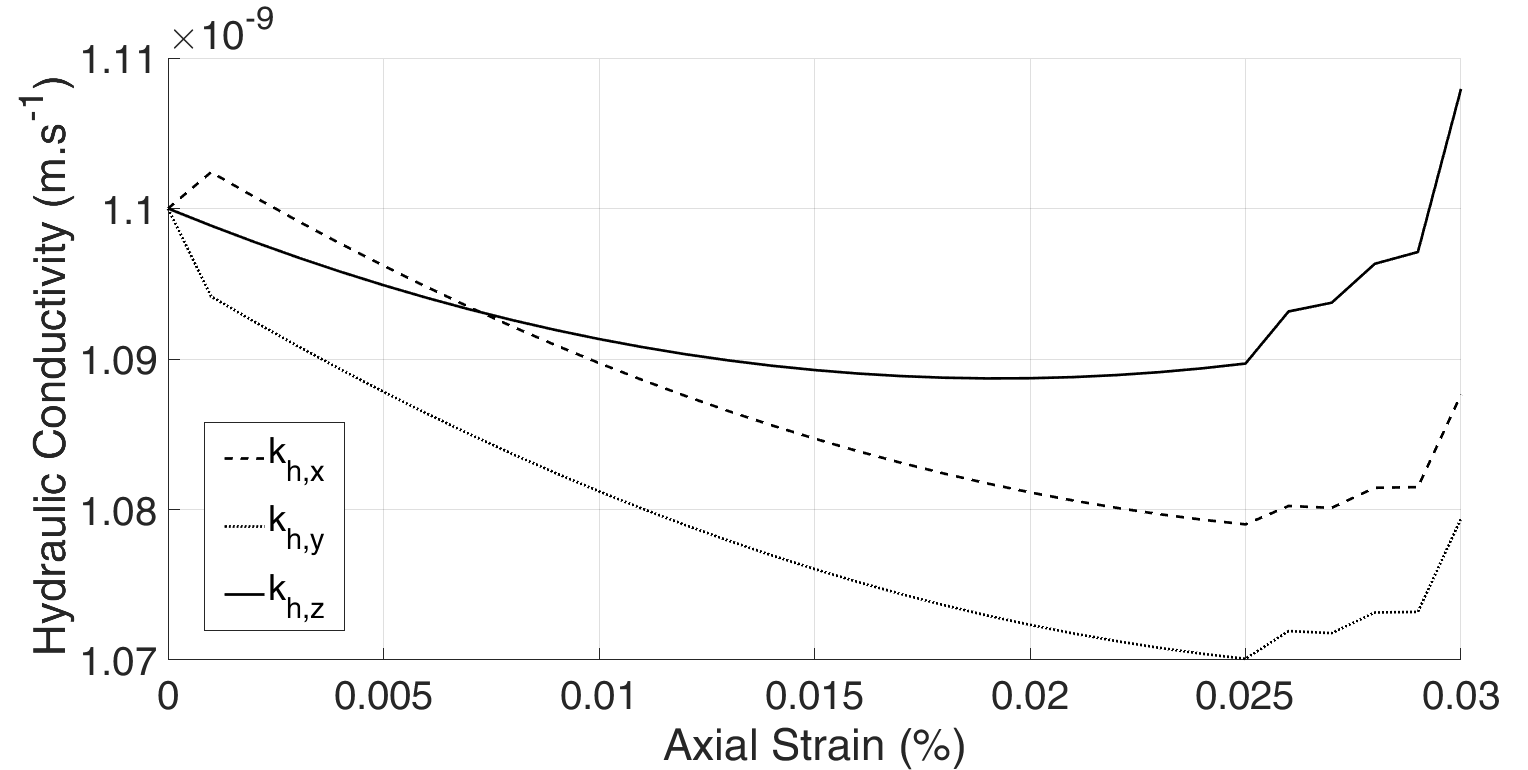
\includegraphics[width=0.75\textwidth]{figures/Amir_ME5_Lattice_Drying_Data.png}
\caption{The change of hydraulic conductivity with applied linear strains}
\label{fig:Amir_ME5_Lattice_Drying_Data}
\end{figure}

\begin{table}[!ht]
\caption{MEX 1-1b: Swelling process, salt clay}
\label{tab:dms-mex1-1b}
\small
\begin{tabular}{R{3cm}|L{7cm}}
\hline
%
Data label & GeomInt | CAU | Swelling process, salt clay\\
URI &  https://nextcloud.ifg.uni-kiel.de/index.php/s/JmZseQqrsbgWNqC (Numerics)\\
Subject  &  Swelling process, Salt Clay\\
Type of data  & executable MATLAB P-file, input parameters\\
Dataquality  &  quality assured data \\
Status of data  &  unprocessed data\\
Dataformat  & txt, MATLAB executable P-file\\
Creators  &  Kiel University, Institute of Geomechanics and Geotechnics, Ludewig-Meyn-Stra\ss e 10, 24118, Kiel\\
Source/Origin & In-house code \\
Publisher  &  Kiel University, Institute of Geomechanics and Geotechnics, Ludewig-Meyn-Stra\ss e 10, 24118, Kiel \\
Rights holders &  Kiel University, Institute of Geomechanics and Geotechnics, Ludewig-Meyn-Stra\ss e 10, 24118, Kiel \\
Contributors &   Kiel University, Institute of Geomechanics and Geotechnics: Amir Shoarian Sattari, Frank Wuttke\\
Time or Period of creation &  2019-2020\\
Language of the content &  English\\
Update policy &  stored data is final\\
Access permissions & full access\\
%
\hline
\end{tabular}
\end{table}